\documentclass[
    aps,
    10pt,
    prd,
    notitlepage,
    onecolumn,s
    tightenlines,
    nofootinbib]{revtex4-1}

\usepackage[linktocpage,breaklinks]{hyperref}
\usepackage[usenames,dvipsnames]{xcolor}

\usepackage{amsmath}
\usepackage{amssymb}
\usepackage{amsfonts}
\usepackage{txfonts}
\usepackage{bm}
\usepackage{stmaryrd}
\usepackage{tensor}
\usepackage{mathrsfs}
\usepackage[utf8]{inputenc}
\usepackage{url}

\usepackage{graphicx}
\usepackage{epsfig}
\usepackage{epstopdf}
\usepackage[normalem]{ulem}

\usepackage{natbib}
\usepackage{hyperref}
\usepackage{cleveref}
\hypersetup{colorlinks=true}

%%%%%%%%%%%%%%%%%%%%%%%%%%%%%%%%%%%%%%%%%%%%%%%%%%%%%%%%%%%%%%%%%%%%%%
\newcommand{\cd}{\nabla}
\newcommand{\dd}{{\rm d}}
\newcommand{\dinf}[1]{\,\dd #1}
\newcommand{\nn}{\nonumber}
\newcommand{\pd}{\partial}
\newcommand{\ii}{{\rm i}}
\newcommand{\calM}{{\cal M}}
%%%%%%%%%%%%%%%%%%%%%%%%%%%%%%%%%%%%%%%%%%%%%%%%%%%%%%%%%%%%%%%%%%%%%%

%%%%%%%%%%%%%%%%%%%%%%%%%%%%%%%%%%%%%%%%%%%%%%%%%%%%%%%%%%%%%%%%%%%%%%
\newcommand{\software}[1]{\texttt{#1}}
%%%%%%%%%%%%%%%%%%%%%%%%%%%%%%%%%%%%%%%%%%%%%%%%%%%%%%%%%%%%%%%%%%%%%%
\begin{document}
\title{Assignment 3}
\date{\today}
\maketitle

In this assignment, the students should work through 3 problems inspired by the assignments in Neil Cornish's MCMC problem sets, in ``MCMC\_cornish\_2020.pdf''.
Additional information in the original assignment is valuable and worth reading through, however, Neil's assignments work through making a full sampler from scratch. 
We will just be using \software{bilby}, so we'll only be doing a version of a subset of those assignments.

These assignments will focus on using MCMC samplers, as opposed to nested samplers, which will be addressed in future assignments.
To accomplish the next two assignments, you should use the \software{emcee} sampler option.
The \software{emcee} sampler operates by using an ensemble algorithm, where multiple chains (called ``walkers'') are all run in parallel. 
The proposal for new positions for a single walker uses the positions of the rest of the ensemble. 
This is a good, general purpose algorithm for many generic problems in Bayesian inference, as it is generally effective and has few tunable parameters.
It's encouraged for the student to read through the algorithm in more detail \href{https://arxiv.org/abs/1202.3665}{here}.

You should also familiarize yourself with the keyword arguments for this sampler in \software{bilby}.
Of particular note are the keyword options ``nsteps'', ``nwalkers'', and ``a'', where ``nsteps'' is the number of steps \emph{per walker}, ``nwalkers'' is simply the number of parallel chains to use, and ``a'' is the parameter that tunes the proposal algorithm.

\begin{enumerate}
\item  In this problem, we will be sampling a set of points $\{x_i\}$ from the student-t probability distribution:
\begin{equation}
p(x| \mu,\nu,\sigma) = \frac{ \Gamma( ( \nu + 1) / 2)}{\Gamma(\nu /2) \sqrt{\nu \pi  } \sigma} \left( 1 + \frac{1}{\nu} \left(  \frac{ x  -\mu}{\sigma} \right)^2 \right)^{- (\nu+1)/2}\,,
\end{equation}
In this problem, the parameters $\mu$, $\nu$, and $\sigma$ are fixed, and are therefore not independent parameters.
As an example, pick the values $\mu=1$, $\nu=3$, and $\sigma=1$.
\begin{enumerate}
\item Write the likelihood class to use the above distribution, similar to what was done in previous assignments.

\item Set up a uniform prior on $\{x_i\}$ between $[-10,10]$, and initiate the sampler with some initial guess at the sampler parameters outlined above.

\item Before running the sampler on the student-t distribution, comment out the likelihood function you have coded up, and have it just return a constant number (any number). 
Run the sampler in this configuration and plot the results. 
Because the likelihood is flat, you should just recover the prior.
This is to ensure that detailed balance is being respected, and is a good check when configuring or modifying MCMC code.
If you do not recover a flat distribution between $[-10,10]$, you're sampler violates detailed balance (meaning there is no guarantee it will produce samples from the desired distribution).

\item Once detailed balance has been verified, you can uncomment out the original likelihood function.
Try sampling with a variety of configurations. 
Take note of how long the chains take to run.
Determine the convergence/efficiency of each configuration in the following ways:
\begin{enumerate}
\item Calculate the autocorrelation (AC) length. There are predefined functions one can use in \href{https://emcee.readthedocs.io/en/stable/user/autocorr/}{\software{emcee}}, or you can use a different approximation:
\begin{equation}
\rho(h) = \frac{\gamma(h)}{\gamma(0)}\,,
\end{equation}
where
\begin{equation}
\gamma(h) = \frac{1}{N-h} \sum_{i=1}^{N-h} \left( x_{i+h} -\bar{x} \right)\left( x_{i} -\bar{x} \right)\,.
\end{equation}
The lag $h$ at which $\rho(h)$ falls to $\sim0.01$ is the AC length.
This quantity approximately tells you how long a chain must iterate to sample an independent point.

\textbf{NOTE:} You should calculate the AC for each walker \emph{separately}. 
You must separate out the data in the final sample file saved by \software{bilby} by walker before doing this analysis. 
These particular diagnostic tools only make sense in the context of a single Markov process, and each walker represents a Markov chain. 
The ensemble as a whole \emph{does not}.
You can calculate the AC for each walker and average them to obtain a more reliable estimate, but each AC must be calculated separately.
Furthermore, if your total chain length for each walker is not $50-100\times$ the AC length, your estimation of the AC length is unreliable. 
This is a numerical estimation, and the error goes down with the number of samples. 

Once you have an estimate of the AC length, you should thin each chain from each walker by this number, so that you only retain ``independent'' samples. 
Once this is done, you can combine the output of each chain.
The number of samples at this point will be the effective number of samples.

\item Plot the chains as a function of iteration. This is commonly referred to as a ``trace plot''.
Again, this should be done for each chain individually (or at least a subset of the chains), but not the whole ensemble at once.

Do the trace plots show large drifts or slow/long oscillations? This indicates poor sampling.

\item Histogram the samples and overlay the student-t distribution (since we know the true distribution, in this case).

\item Repeat the problem replacing the uniform prior with the custom prior that you wrote in the previous assignment.
\end{enumerate}
To compare each configuration, compare the effective number of samples, the quality of the trace plot, the accuracy of the histogram, and the time to sample those points.
\item Find a reliable configuration to draw $10^3 - 10^4$ independent samples, and save these samples in a file for the next assignment.
\item Repeat the above steps for $\mu=-2$, $\nu = 10$, and $\sigma=7$, and notice how different distributions might require different configurations.
\end{enumerate}

\item With the code from the previous problem, produce a large number of independent samples with $\mu=1$, $\nu=3$, and $\sigma=1$.
We will now flip the problem, and use these independent samples as our ``observable'', and try to infer the parameters of the student-t distribution that produced the samples.
Now, $\{x_i\}$ is fixed and $\nu$, $\mu$, and $\sigma$ are the parameters.
We will use the new likelihood function
\begin{equation}
p(\{x_i\}|\mu,\nu,\sigma) = \prod_{i=1}^{N} \frac{ \Gamma( ( \nu + 1) / 2)}{\Gamma(\nu /2) \sqrt{\nu \pi  } \sigma} \left( 1 + \frac{1}{\nu} \left(  \frac{ x_i  -\mu}{\sigma} \right)^2 \right)^{- (\nu+1)/2}\,,
\end{equation}
for dataset $\{x_i\}$ of length $N$.
Note that this product could be very large if $N$ is large, so it would be wise to work in log space as early in the calculation as possible.
Take the prior to be uniform with $\nu \in [0.1,10]$, $\mu \in [-5,5]$, and $\sigma \in [0.1,10]$.

\begin{enumerate}
\item Sample with a $N=100$, and plot the convergence statistics from the previous problem for different configurations of the sampler.
Instead of a single histogram, you can plot a ``corner plot'', either constructed from scratch or using a library like \href{https://corner.readthedocs.io/en/latest/}{\software{corner}}. This will show the 2D covariance for each parameter, as well as the 1D marginalized posterior on each parameter.
Trends in the covariance plots show which parameters are degenerate.
In real data analysis problems that are more complex, one may wish to reparameterize the problem so as to reduce covariances and make the sampling process faster.
\item Repeat this process with $N=1000$.
Larger datasets lead to smaller errors, as long as the error in parameter estimation is dominated by statistical error.
\end{enumerate}
\item Now we will use a more complicated distribution, where parallel tempering (PT) will hopefully improve the convergence.
The new likelihood function is 
\begin{equation}
\pi(x,y) = \frac{16}{3\pi} \left( e^{-x^2 - ( 9+4x^2 + 8 y )^2} + \frac{1}{2} e^{-8x^2 - 8(y-2)^2} \right)\,.
\end{equation}
A sample MCMC output of this distribution is shown in Fig.~\ref{fig:rosen}
\begin{figure}
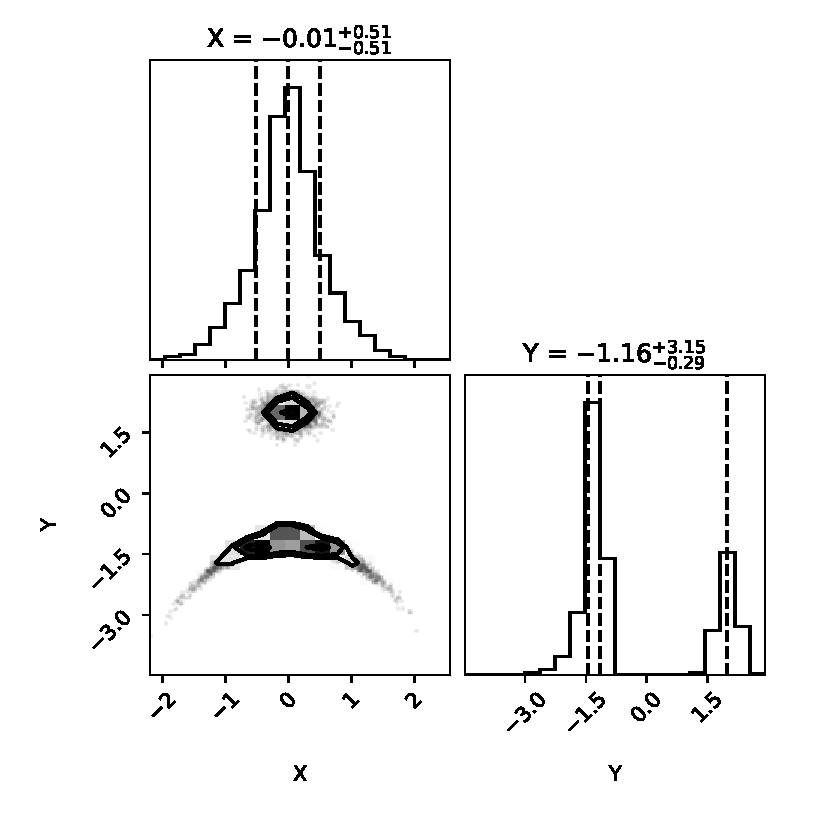
\includegraphics[width=.5\linewidth]{rosen.pdf}
\caption{Target distribution for problem 3. Notice the multimodality of the distribution, and the strong covariance between the parameters.}\label{fig:rosen}
\end{figure}

Please read through the parallel tempering section in Assignment 4 of ``MCMC\_cornish\_2020.pdf'' for an overview of how parallel tempering works. 
\begin{enumerate}
\item 
Use \software{emcee} to try and sample from the distribution, with different configurations. Is the sampler effectively exploring the full posterior in a reasonable time? In particular, pay attention to the trace plot of the individual chains.
If each chain only explores one mode, the AC calculation shouldn't be absolutely trusted.
\item 
We will now use a PTMCMC sampler to sample the same distribution.
There are two choices prebuilt in \software{bilby}, one of which is called \href{https://github.com/jellis18/PTMCMCSampler/}{\software{ptmcmcsampler}}.
This code is a more standard approach, using the traditional Metropolis-Hastings algorithm with a single cold chain. 
This means that the output can be treated as a single Markov process, and no sorting is required.
Feel free to explore the different proposals it uses, although the default is fine.
Be sure to write out the full chain without thinning, so that we can verify the convergence ourself (normally, it would probably be fine to let bilby do this itself).
You can also explore the ``burn'' parameter, which controls how many initial samples to throw away before storing the output. 
This is done to excise the samples where the sampler is finding a maximum and reaching equilibrium.
If these steps are not removed, your AC calculation might not be accurate.
Normally, it would be okay to allow the sampler to determine this, but it's always a good idea to look for transitory behavior in the trace plots when running an MCMC.
For more complex problems, the algorithms do not always identify the burn-in period correctly.
You can set this parameter to a low value, and you will probably see some behavior early in the chain to indicate its ``burning in''.

Another sampler using PT is \href{https://github.com/willvousden/ptemcee}{\software{ptemcee}}.
This sampler is a generalization of \software{emcee} that runs a set of walkers at different temperatures, and uses the PT algorithm algorithm to propose swaps.
It is normally the sampler of choice, as the combination of ensemble proposals and PT is generally effective, but there doesn't currently appear to be a way to save the full output, without the sampler doing post-processing.
I recommend it for general use, but for this assignment, you should conduct the convergence analysis yourself.
If you use this down the road, you will have to experiment with how to determine convergence if you do not trust the convergence estimates by \software{bilby}.

\end{enumerate}

\end{enumerate}

\end{document}
